\chapter{Jump the Obstacles}

With this project you will create a popular computer game. The player will control a character using the arrow keys. His goal will be to cross the course without touching the obstacles. In cases where it touches them, it will start from the beginning. If he manages to pass the entire route, he moves to the next level.

\begin{figure}[H]
   \centering
   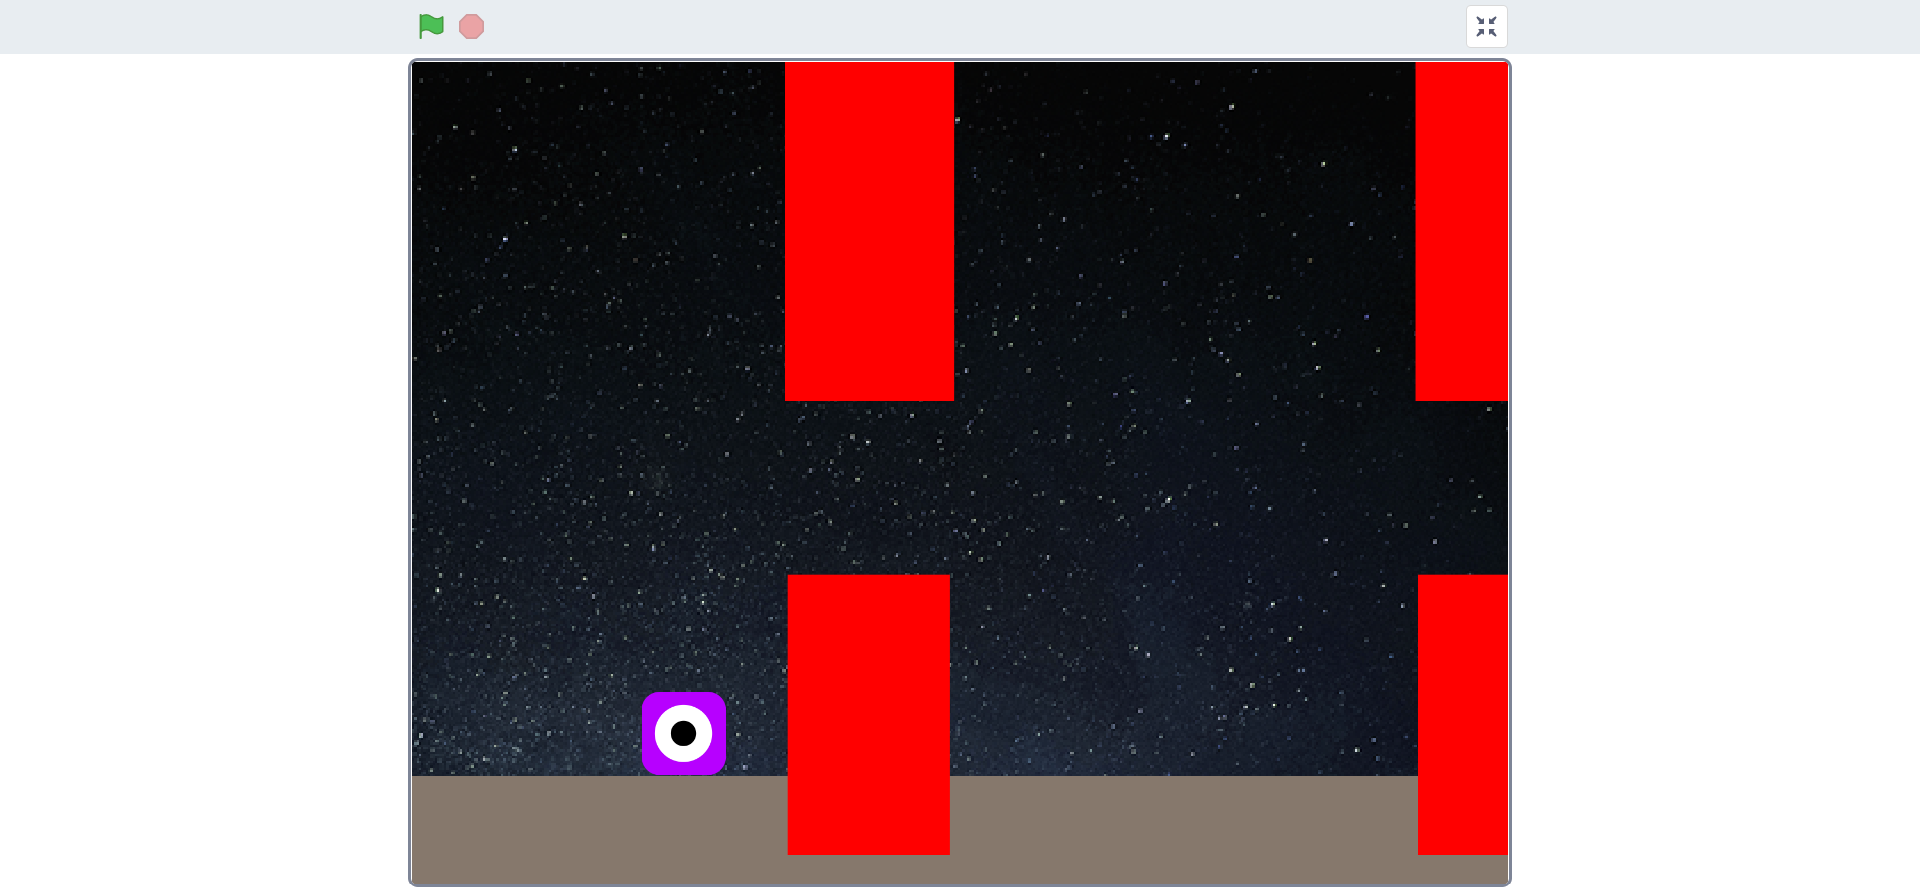
\includegraphics[width=1.0\linewidth,height=0.5\linewidth]{fig140001.png}
   \caption{Jump the obstacles}
\label{fig140001}
\end{figure}

\section{Creating the Design}
The first step in creating the game will be adding the appropriate characters and background. For the game character, you can choose from ready-made characters in Scratch. Another option is to draw it to make your game more interesting. Using the drawing tools you can create your character (Fig. \ref{fig140002}). In this project I will demonstrate how to create an effect when the character moves. For this purpose, one more suit should be added to it.

\begin{figure}[H]
   \centering
   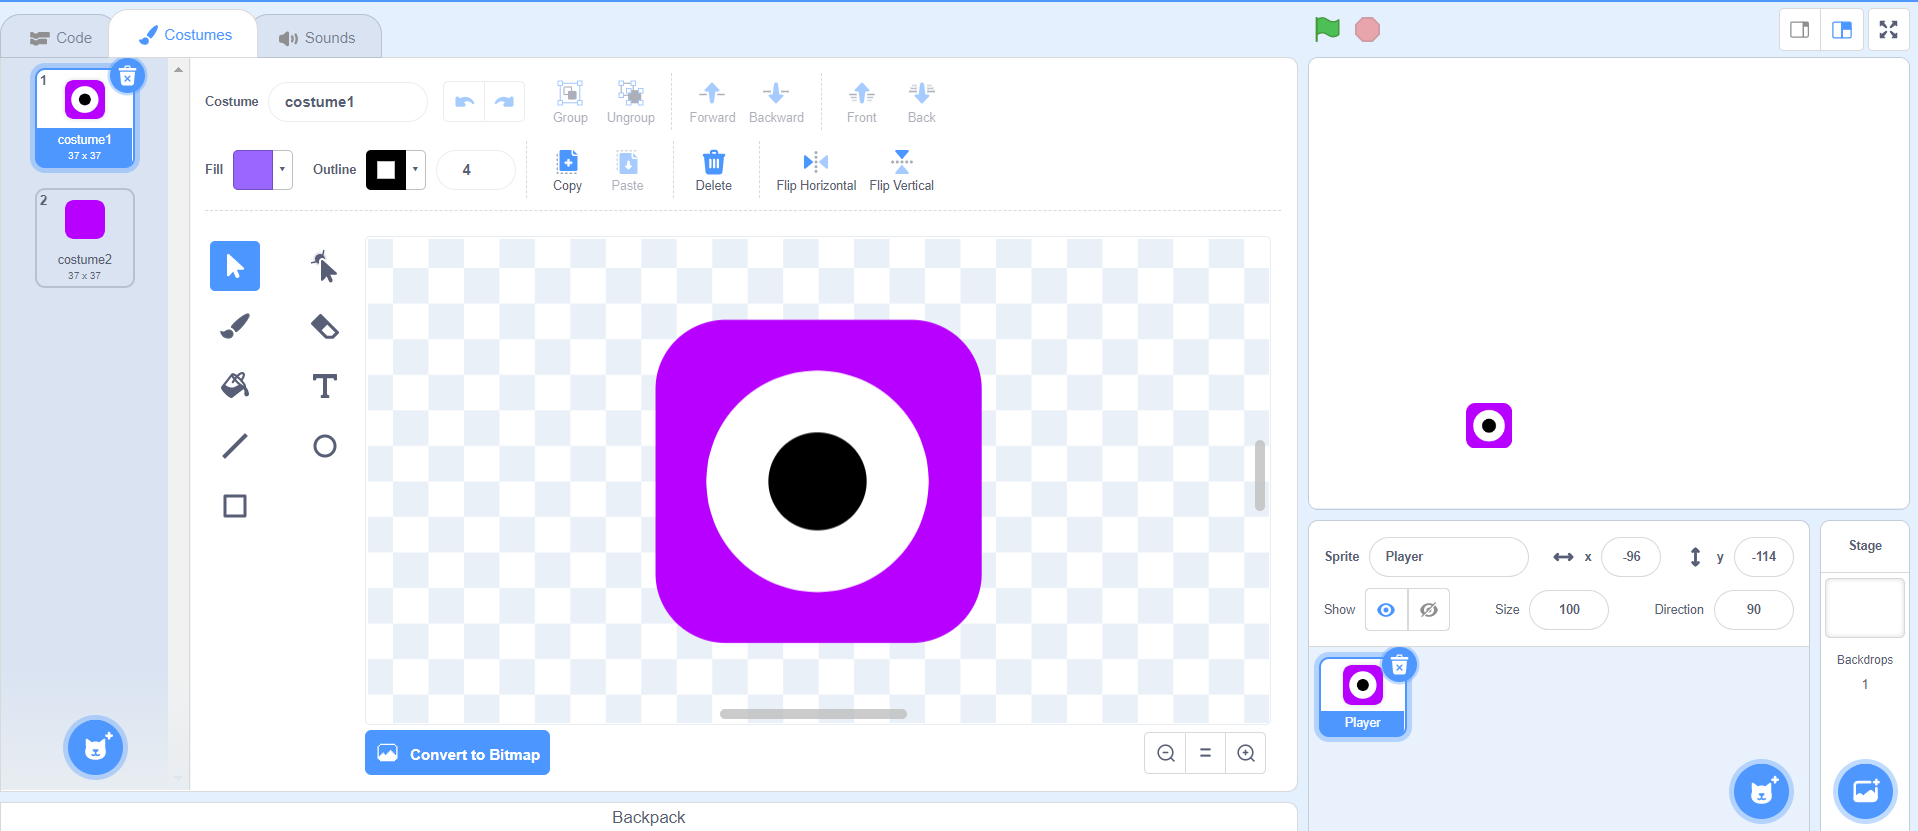
\includegraphics[width=1.0\linewidth,height=0.5\linewidth]{fig140002.png}
   \caption{Adding Main Character}
\label{fig140002}
\end{figure}

The game will need one character to be in the lower part of the track. This is a revenge hero that will serve as a reference point. The purpose of the purple character is to move on it. Create it using the drawing tools.

\begin{figure}[H]
   \centering
   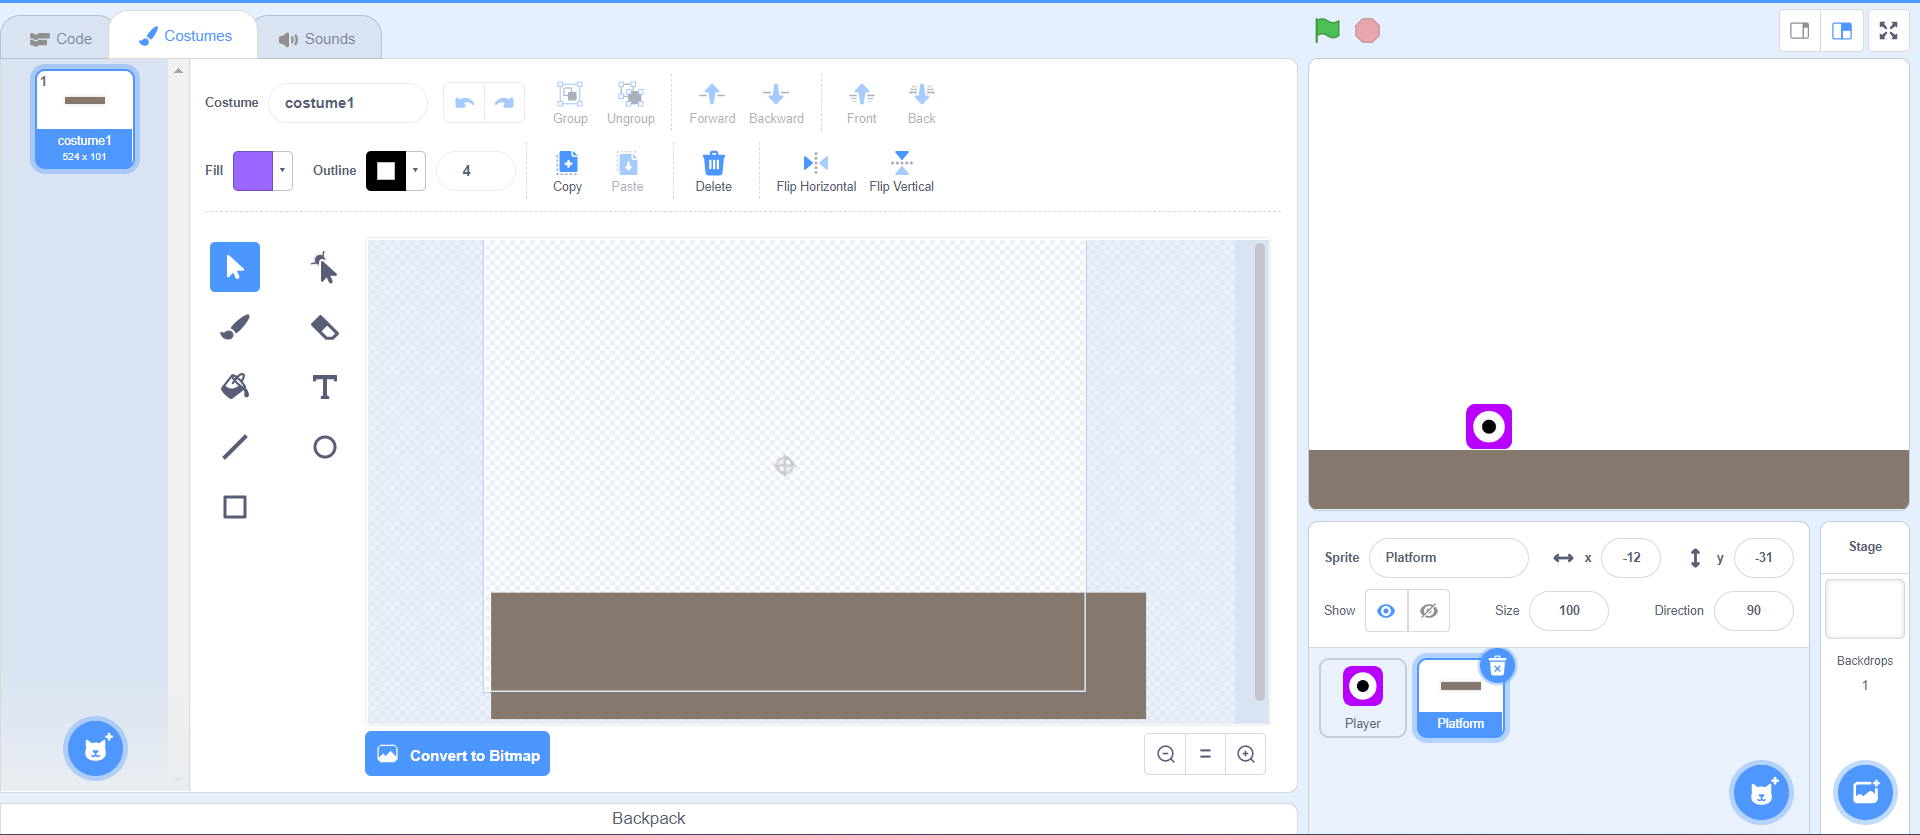
\includegraphics[width=1.0\linewidth,height=0.5\linewidth]{fig140003.png}
   \caption{Adding the supporting character}
\label{fig140003}
\end{figure}

The last character to add is the one for the obstacles. It must be drawn again with the auxiliary tools. To have more levels in the game, add more costumes to your character. When your purple character crosses the track, ie. reach the rightmost point of the screen, then that character will change his costume, which means the player will go to the second level.

\begin{figure}[H]
   \centering
   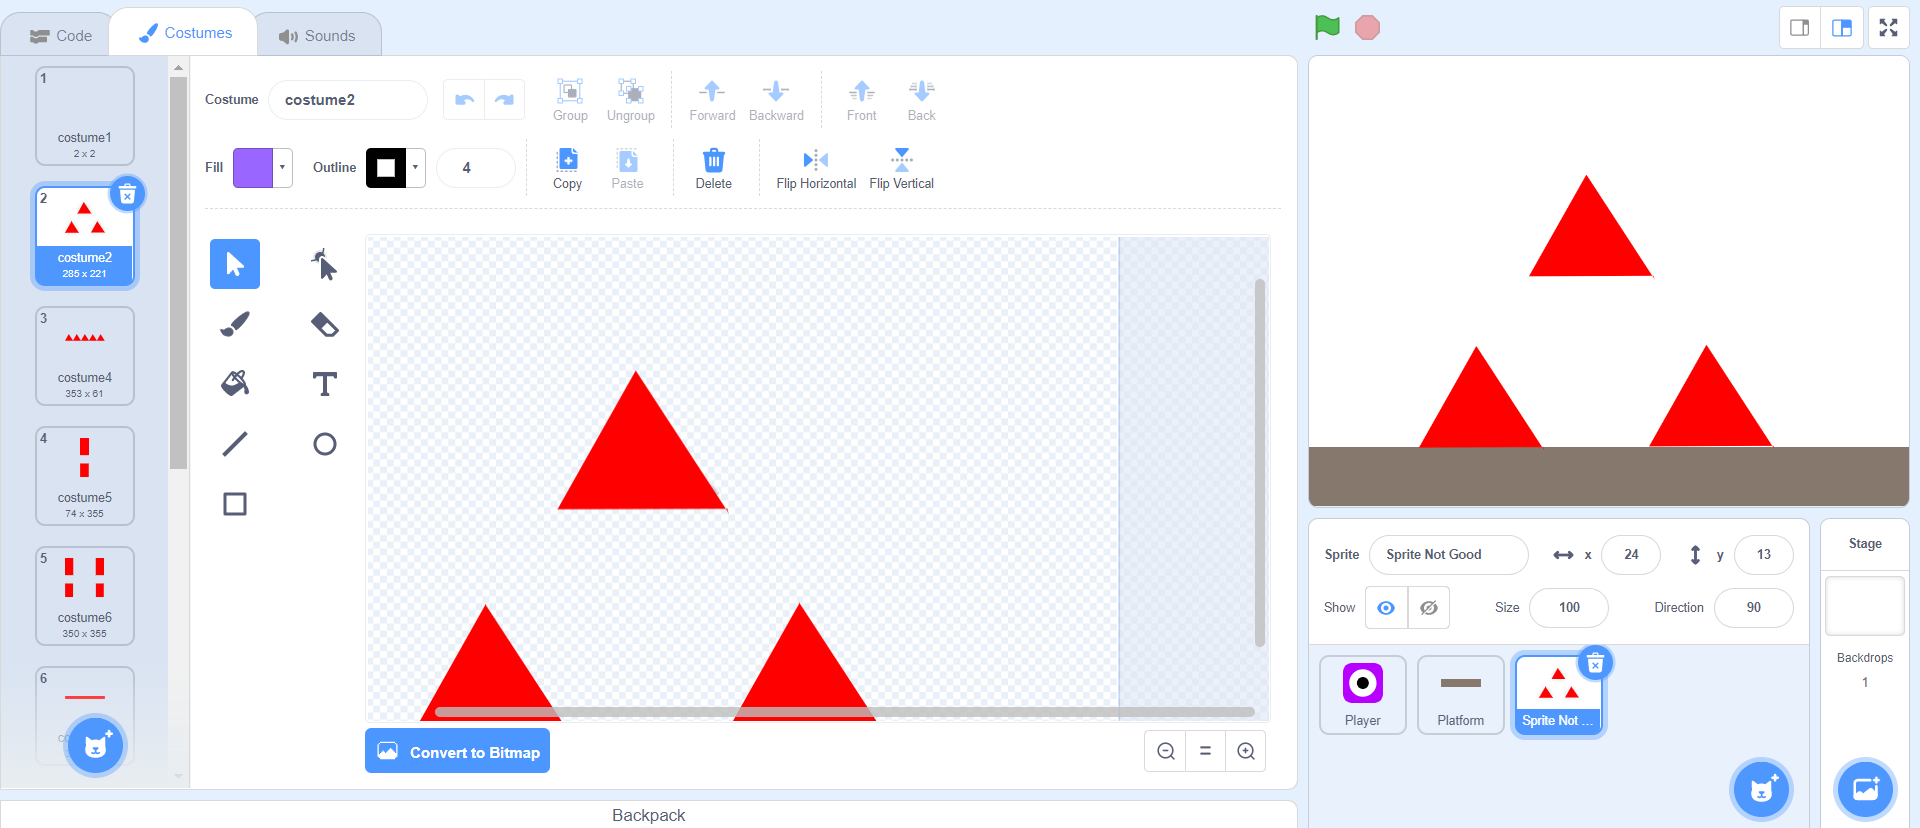
\includegraphics[width=1.0\linewidth,height=0.5\linewidth]{fig140004.png}
   \caption{Add obstacles}
\label{fig140004}
\end{figure}

To make the game more attractive, add a suitable background. Also, like the characters, you can choose it from the ready-made ones in Scratch or draw it yourself using the tools.

\begin{figure}[H]
   \centering
   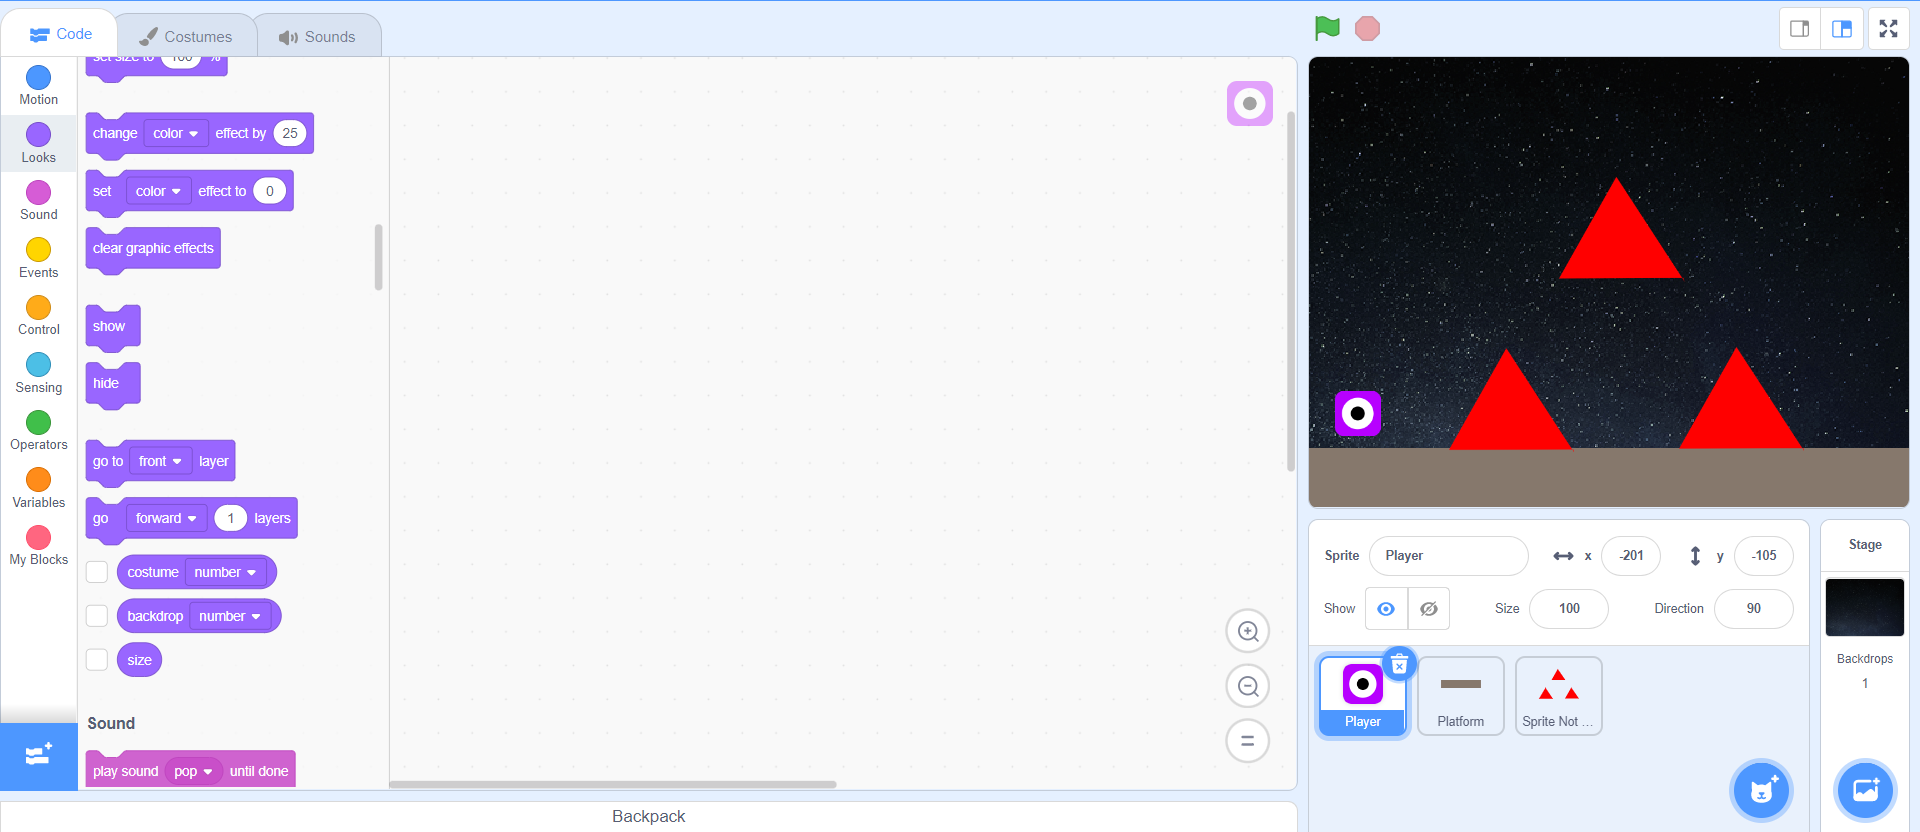
\includegraphics[width=1.0\linewidth,height=0.5\linewidth]{fig140005.png}
   \caption{Add background}
\label{fig140005}
\end{figure}

\section{Programming Character Movement}

The main code you need to add is located in the character you will be controlling, in this case the purple character. In this game you will need 3 variables - xVel, yVel and jump. From the Variables section, select the Make a Variable option and add the variables with the appropriate names. To prevent them from appearing during gameplay, you can remove their ticks.

\begin{figure}[H]
   \centering
   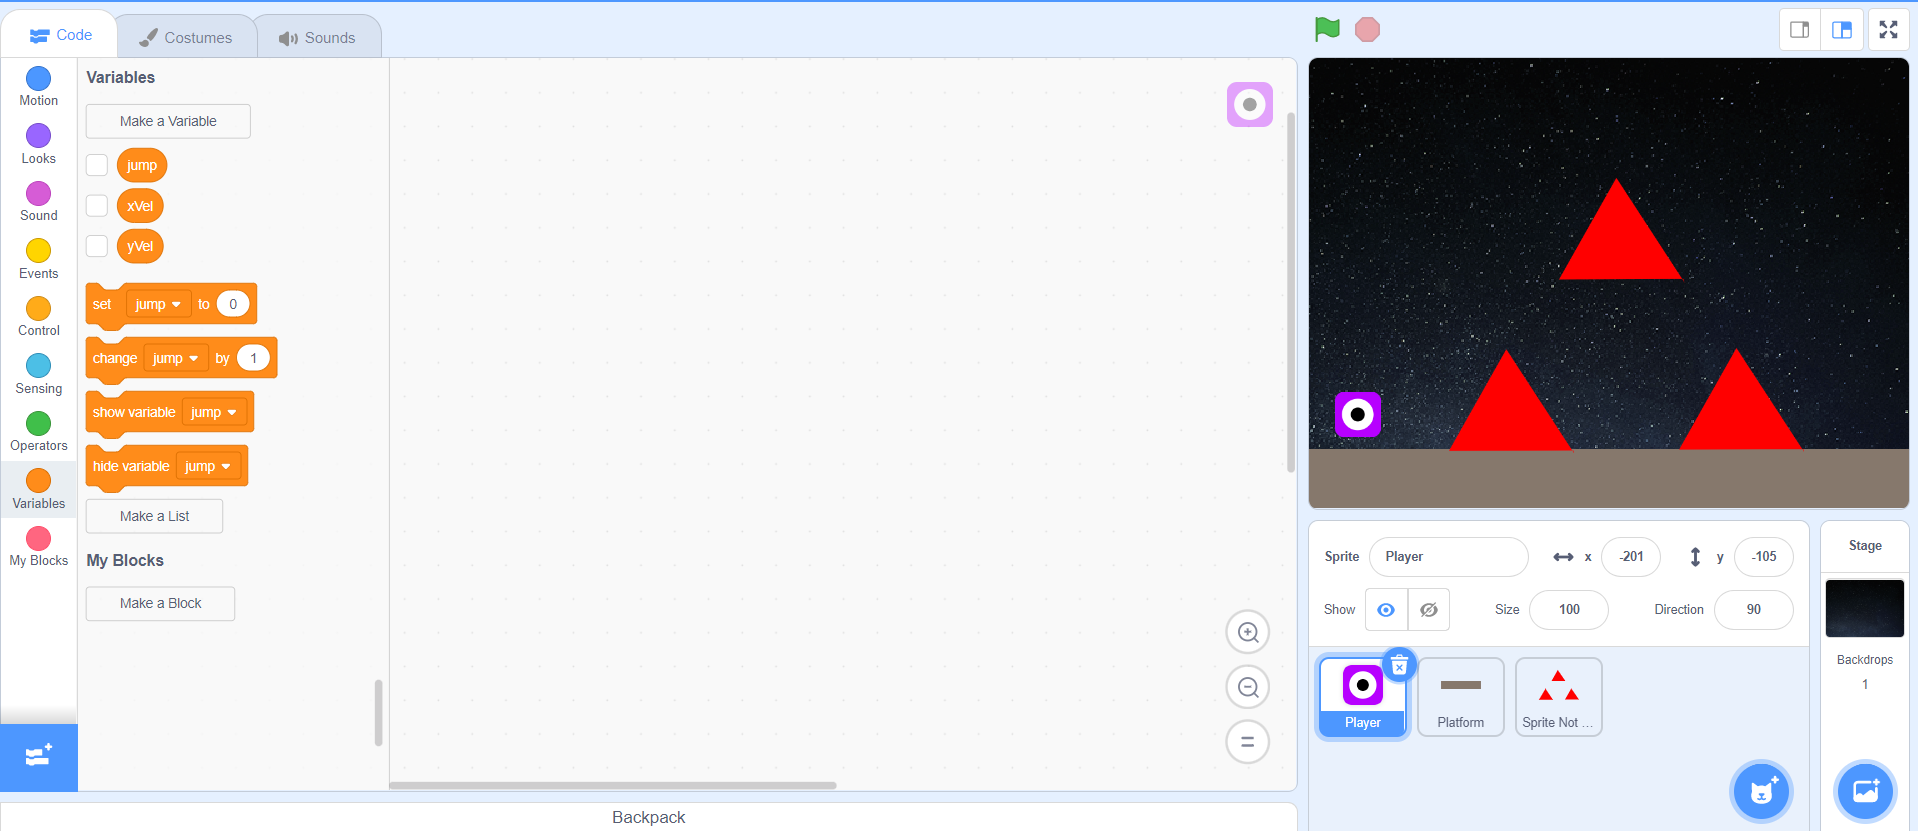
\includegraphics[width=1.0\linewidth,height=0.5\linewidth]{fig140006.png}
   \caption{Adding the variables}
\label{fig140006}
\end{figure}

At the beginning of the game, the value of these variables should be equal to 0. To make the game more interesting, the character's position will be in the middle part of the screen. When the game starts he will drop down to the platform.

\begin{figure}[H]
   \centering
   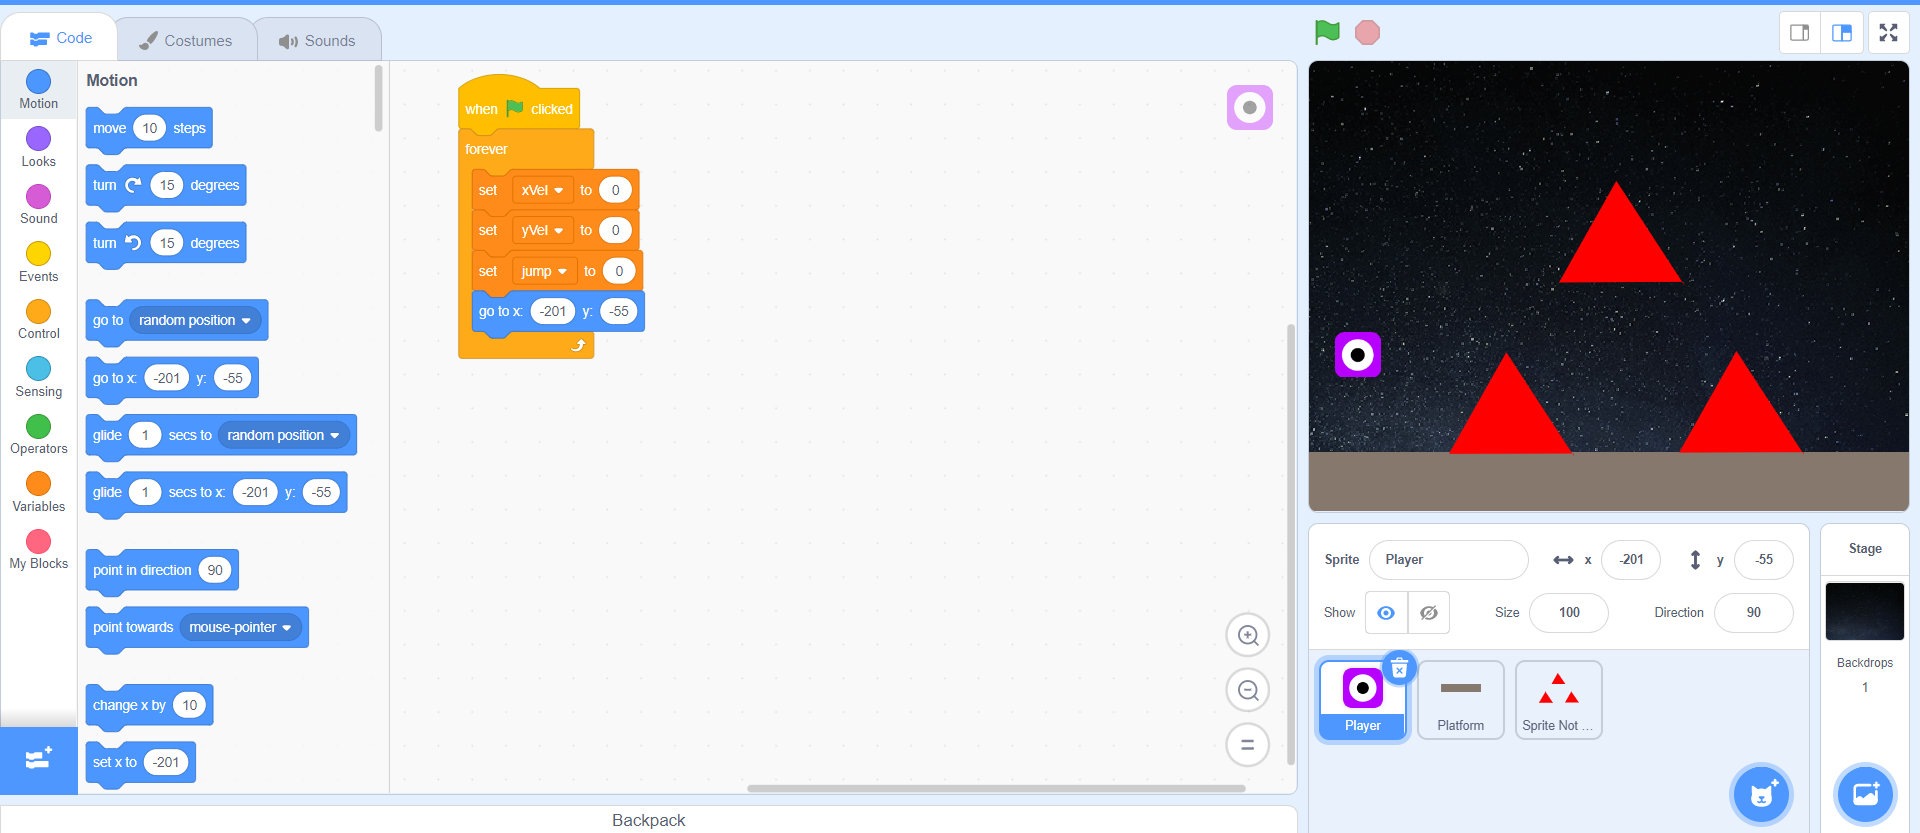
\includegraphics[width=1.0\linewidth,height=0.5\linewidth]{fig140007.png}
   \caption{Initialize variables}
\label{fig140007}
\end{figure}

The character must move until it reaches the right side of the screen or until the character touches an obstacle. For this purpose, the first statement you need to add is a repeat until block. The conditions you need to add are two that are separated by the OR operator. The first condition is that the character's x position is greater than 240, which is the end of the screen. The second condition is to touch the red character.

\begin{figure}[H]
   \centering
   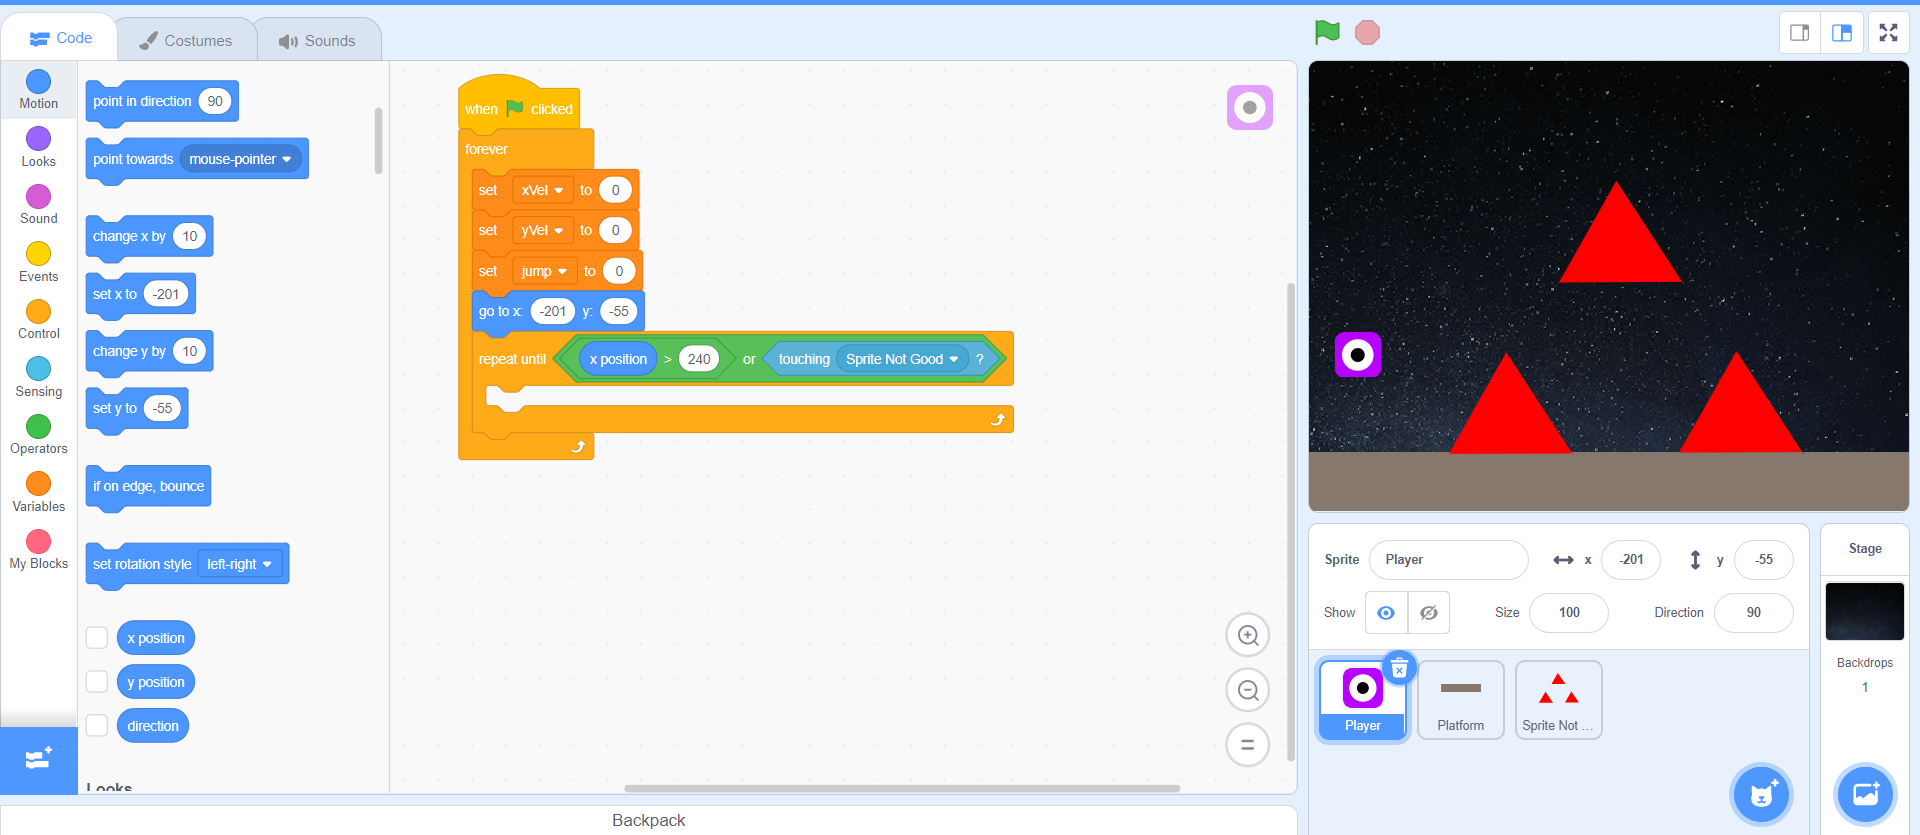
\includegraphics[width=1.0\linewidth,height=0.5\linewidth]{fig140008.png}
   \caption{Loop with character movement condition}
\label{fig140008}
\end{figure}

To move the character left and right you will use the xVel variable. From the variable section, the change xVel by statement is needed. From the operators section, select the one to subtract. On one side put the instruction for key right arrow pressed, and on the right arrow key left arrow pressed. This statement will set a value to the variable. All that remains is to add the change x by instruction and place the variable. So if you start the game, the character will move very fast left and right. For this add the instruction set xVel to xVel * 0.9. Start the game to test how the character moves left and right.

\begin{figure}[H]
   \centering
   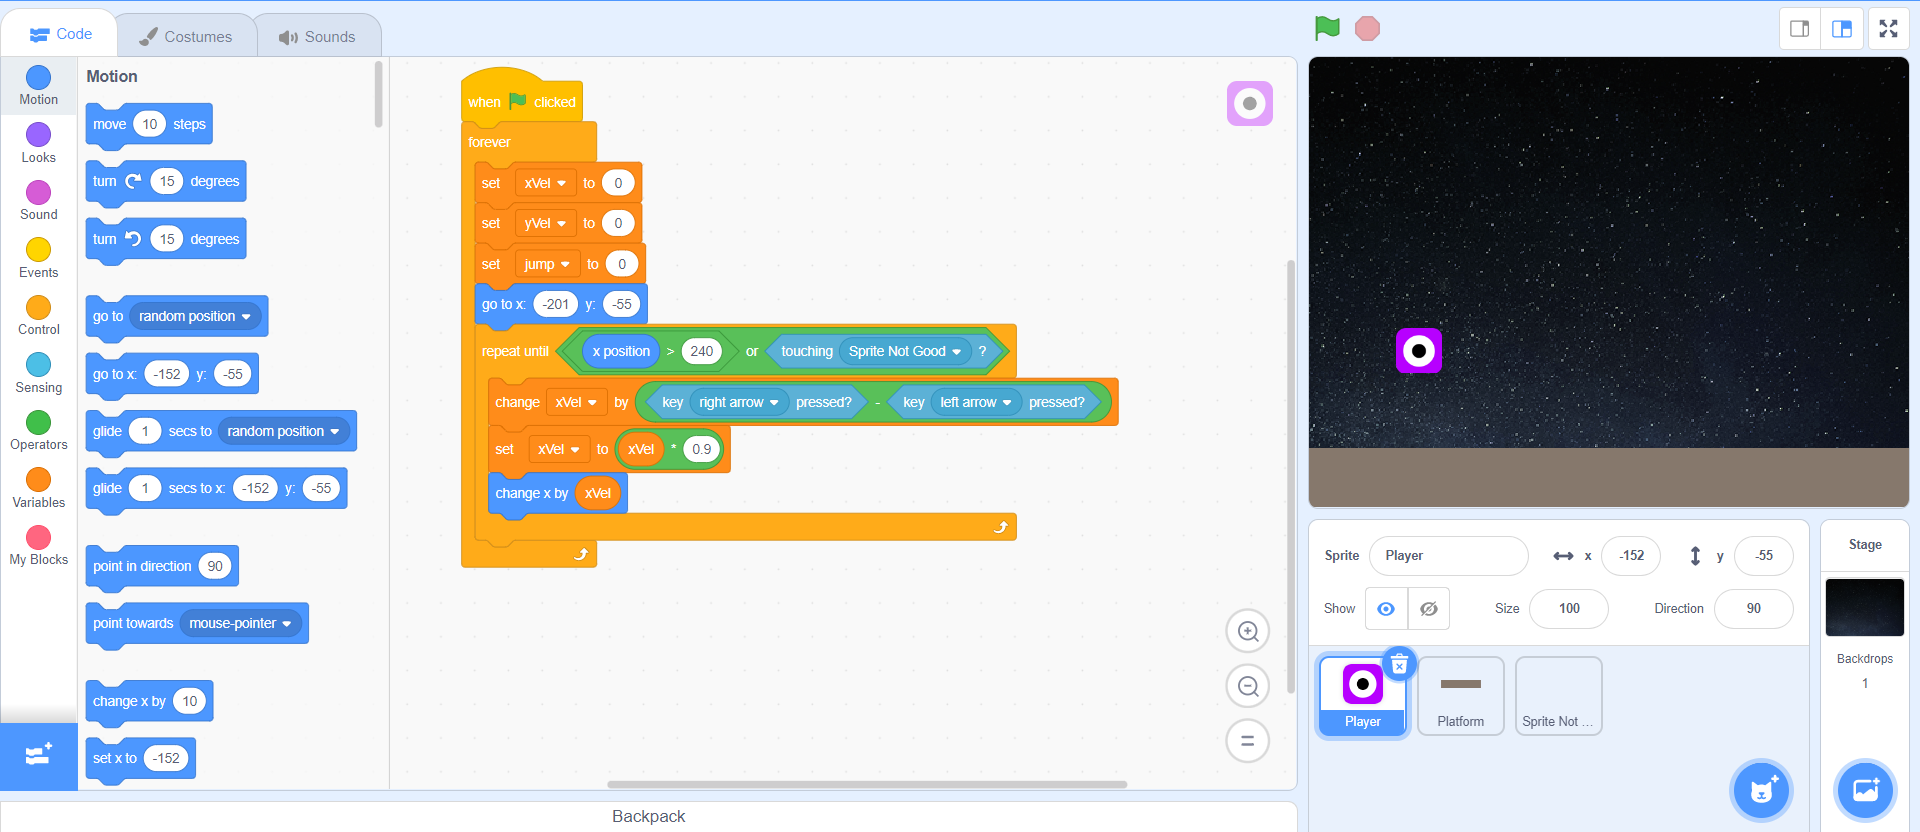
\includegraphics[width=1.0\linewidth,height=0.5\linewidth]{fig140009.png}
   \caption{Character movement left and right}
\label{fig140009}
\end{figure}

You must program the character to jump In the first part, you will program when the game starts or another level that the character from the initial position goes down to the platform. To do this, you need to change the variable yVel to -1 and use the statement change y by with the value variable. Next is the check if it touches the platform. If the condition is met, then the value of the variable yVel should be set to 0. So the only problem will be that the character will not stop moving when it touches the platform, because the main loop will spin one more time, because not ready condition is not met. For this, the y position must be changed by yVel multiplied by -1.

\begin{figure}[H]
   \centering
   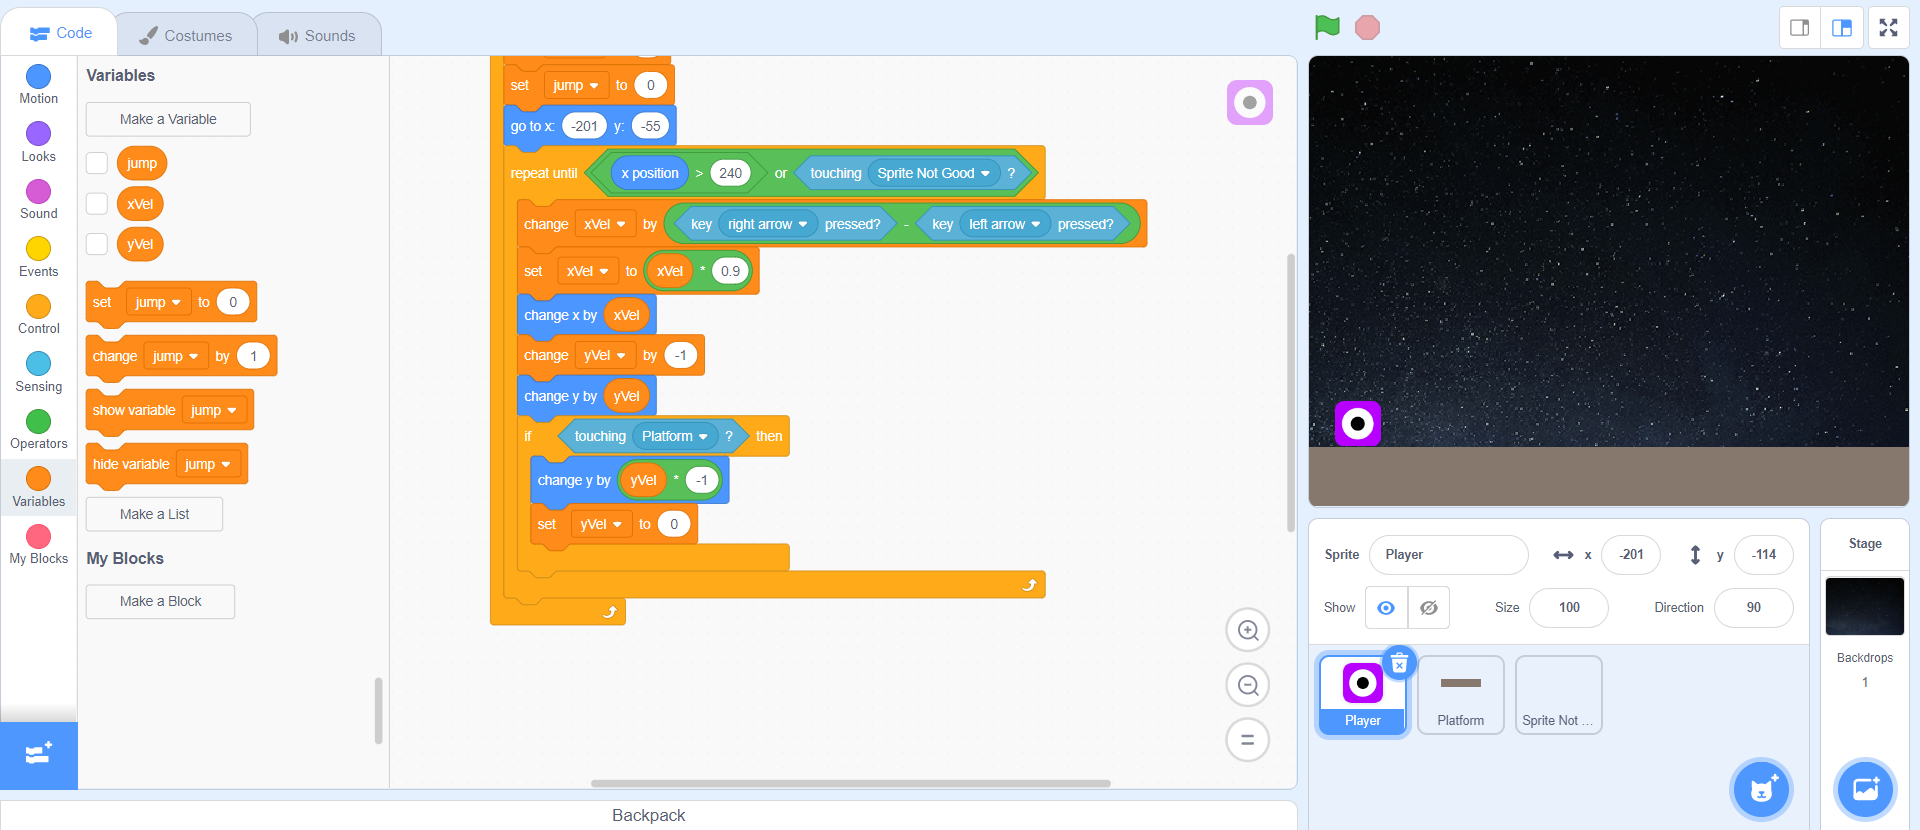
\includegraphics[width=1.0\linewidth,height=0.5\linewidth]{fig140010.png}
   \caption{Moving Character Down}
\label{fig140010}
\end{figure}

The last part of creating the purple character's movement algorithm will be adding the jumps. If the player presses the up arrow, then the jump variable will be equal to 1. In any of the other cases, it should be equal to 0, which means that the character will not jump. First you need to add a check before making yVel equal to 0. This check should check if yVel is less than 0 then the character should not jump.

\begin{figure}[H]
   \centering
   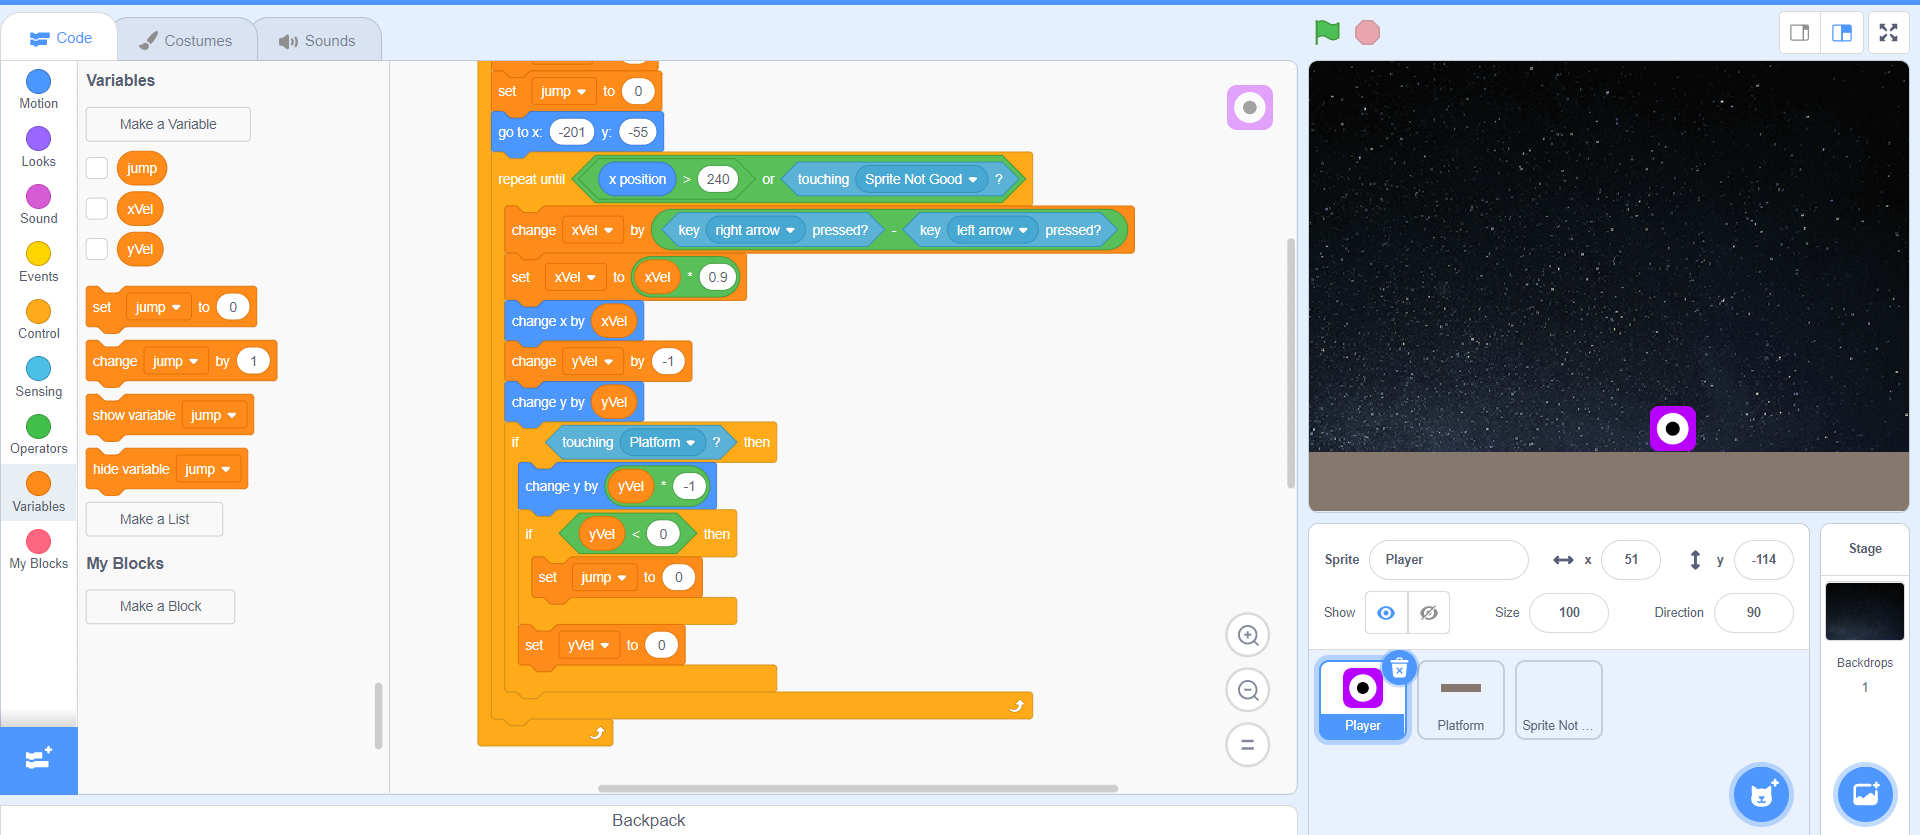
\includegraphics[width=1.0\linewidth,height=0.5\linewidth]{fig140011.png}
   \caption{Checking when character doesn't jump}
\label{fig140011}
\end{figure}

There is also a check to see if the player has pressed the up arrow. If it is and the character is not jumping, then yVel should be changed to a positive number and the jump variable should be set to 1. Playtest to see how your character jumps and moves left and right.

\begin{figure}[H]
   \centering
   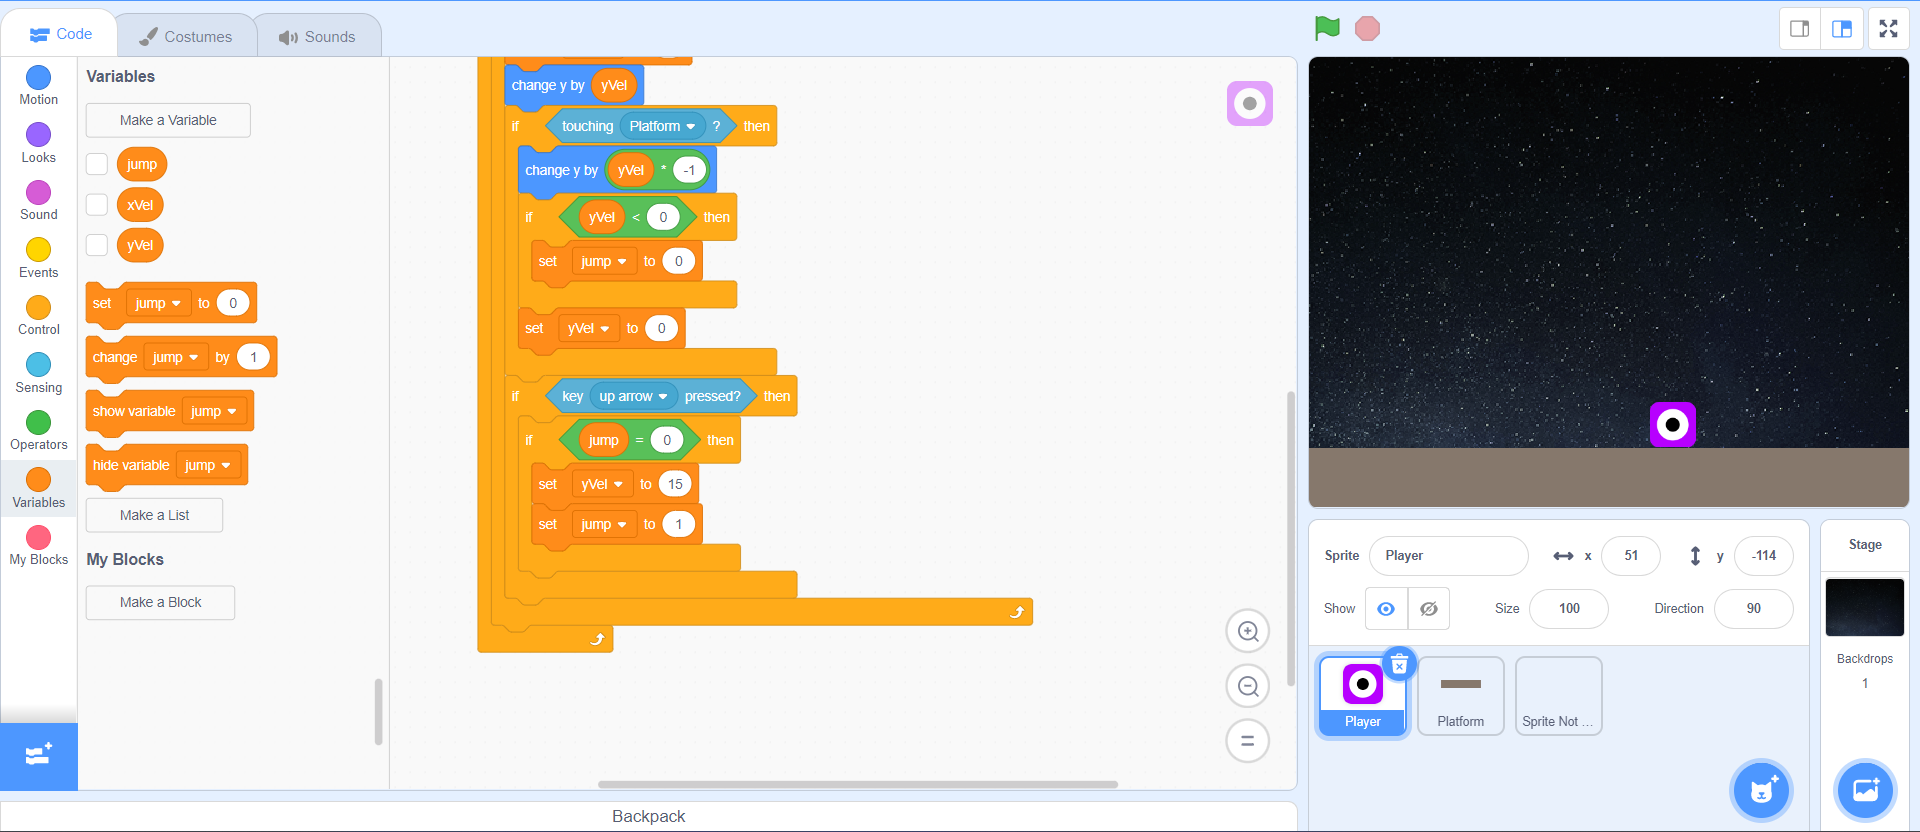
\includegraphics[width=1.0\linewidth,height=0.5\linewidth]{fig140012.png}
   \caption{Hero jump when pressing up arrow}
\label{fig140012}
\end{figure}

\section{Creating an effect when the character moves}

After you have finished moving the character, you can add additional instructions to create an effect when the character moves. After checking for the pressed up arrow, add the create clone of myself statement. The reason for this is that a clone of that character will be created, but with his second costume. For this add a new instruction which is When I start as a clone. Then the character's costume should be changed, it should be his second. Add a loop that repeats 10 times. Inside the loop, reduce the size of the clone character and add a transparent effect. After the cycle, delete the clone. Test the game to see what effect is added when you move.

\begin{figure}[H]
   \centering
   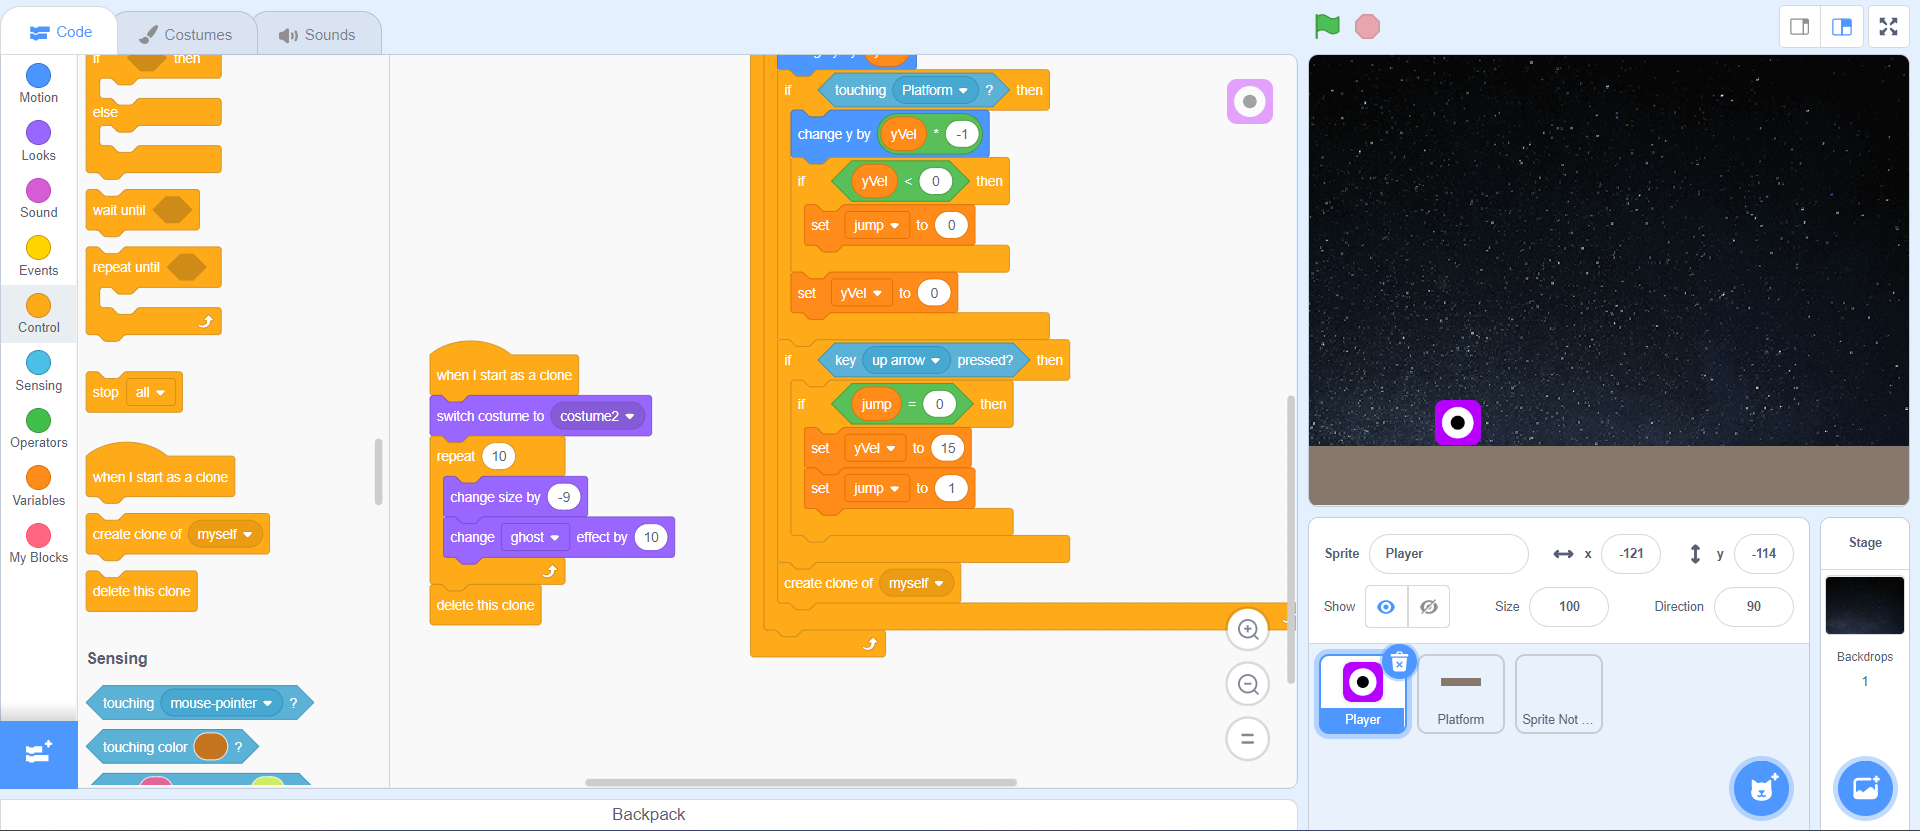
\includegraphics[width=1.0\linewidth,height=0.5\linewidth]{fig140013.png}
   \caption{Add motion effect}
\label{fig140013}
\end{figure}

\section{Go to next level}

In the last step, you need to add instructions for the character to be able to move to the next level. For this purpose, in the main character, add the check if he has reached the end of the screen. If it is, then let it send a message.

\begin{figure}[H]
   \centering
   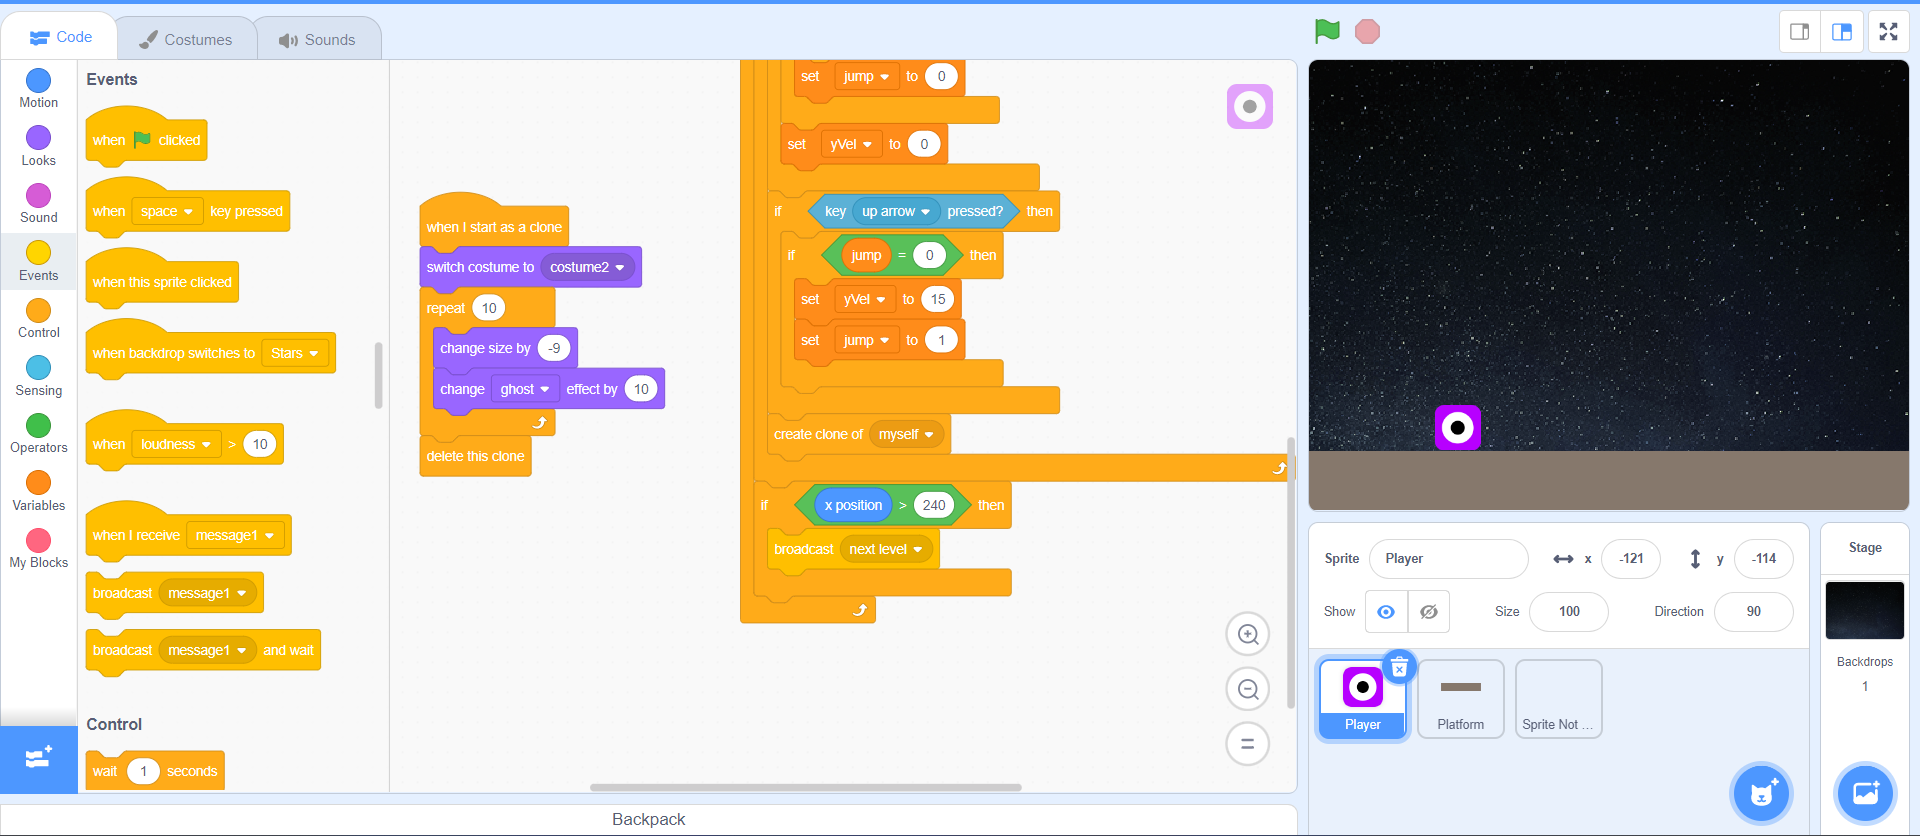
\includegraphics[width=1.0\linewidth,height=0.5\linewidth]{fig140014.png}
   \caption{Send Next Level Message}
\label{fig140014}
\end{figure}

Choose the hero with the red obstacles. Add the event when the game starts, then the character should be in his original costume. Also add a second event when he gets the next level message, he then has to change his suit. Start the game and have fun.

\begin{figure}[H]
   \centering
   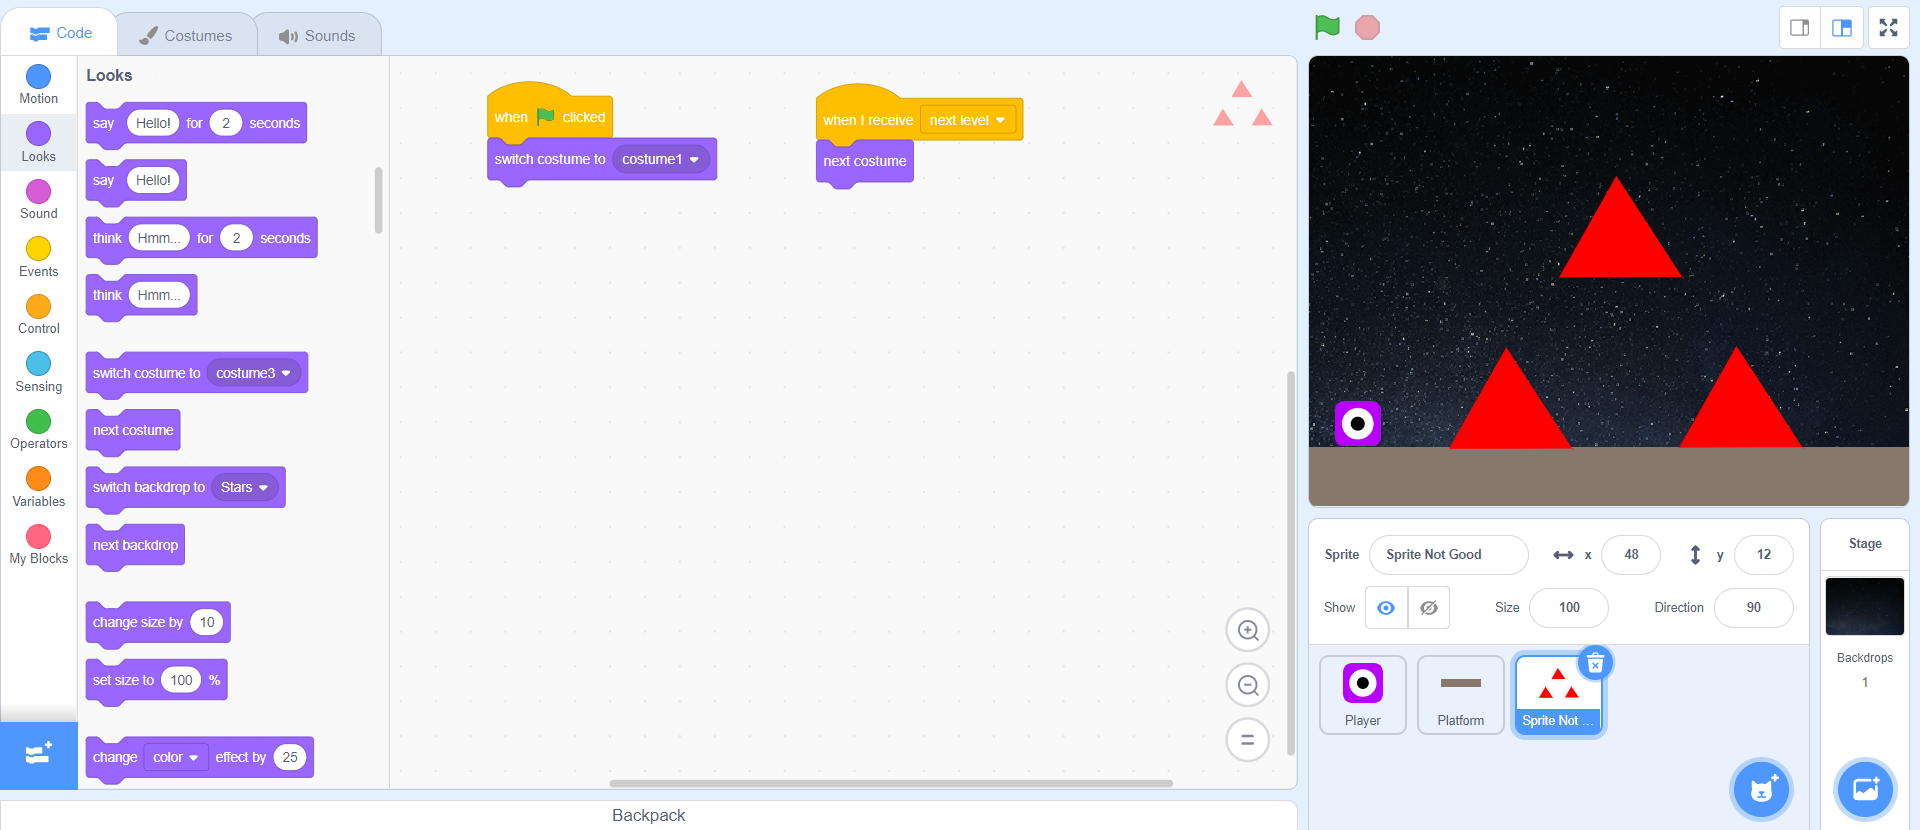
\includegraphics[width=1.0\linewidth,height=0.5\linewidth]{fig140015.png}
   \caption{Go to next level}
\label{fig140015}
\end{figure}
